\begin{figure*}[!t]
    \centering
    % Define specific dimensions to ensure uniformity
    \newcommand{\figwidth}{0.49\columnwidth}
    \newcommand{\figheight}{3.3cm} % Adjust this value until the aspect ratio looks natural
        \begin{subfigure}[b]{\figwidth}
        \centering
        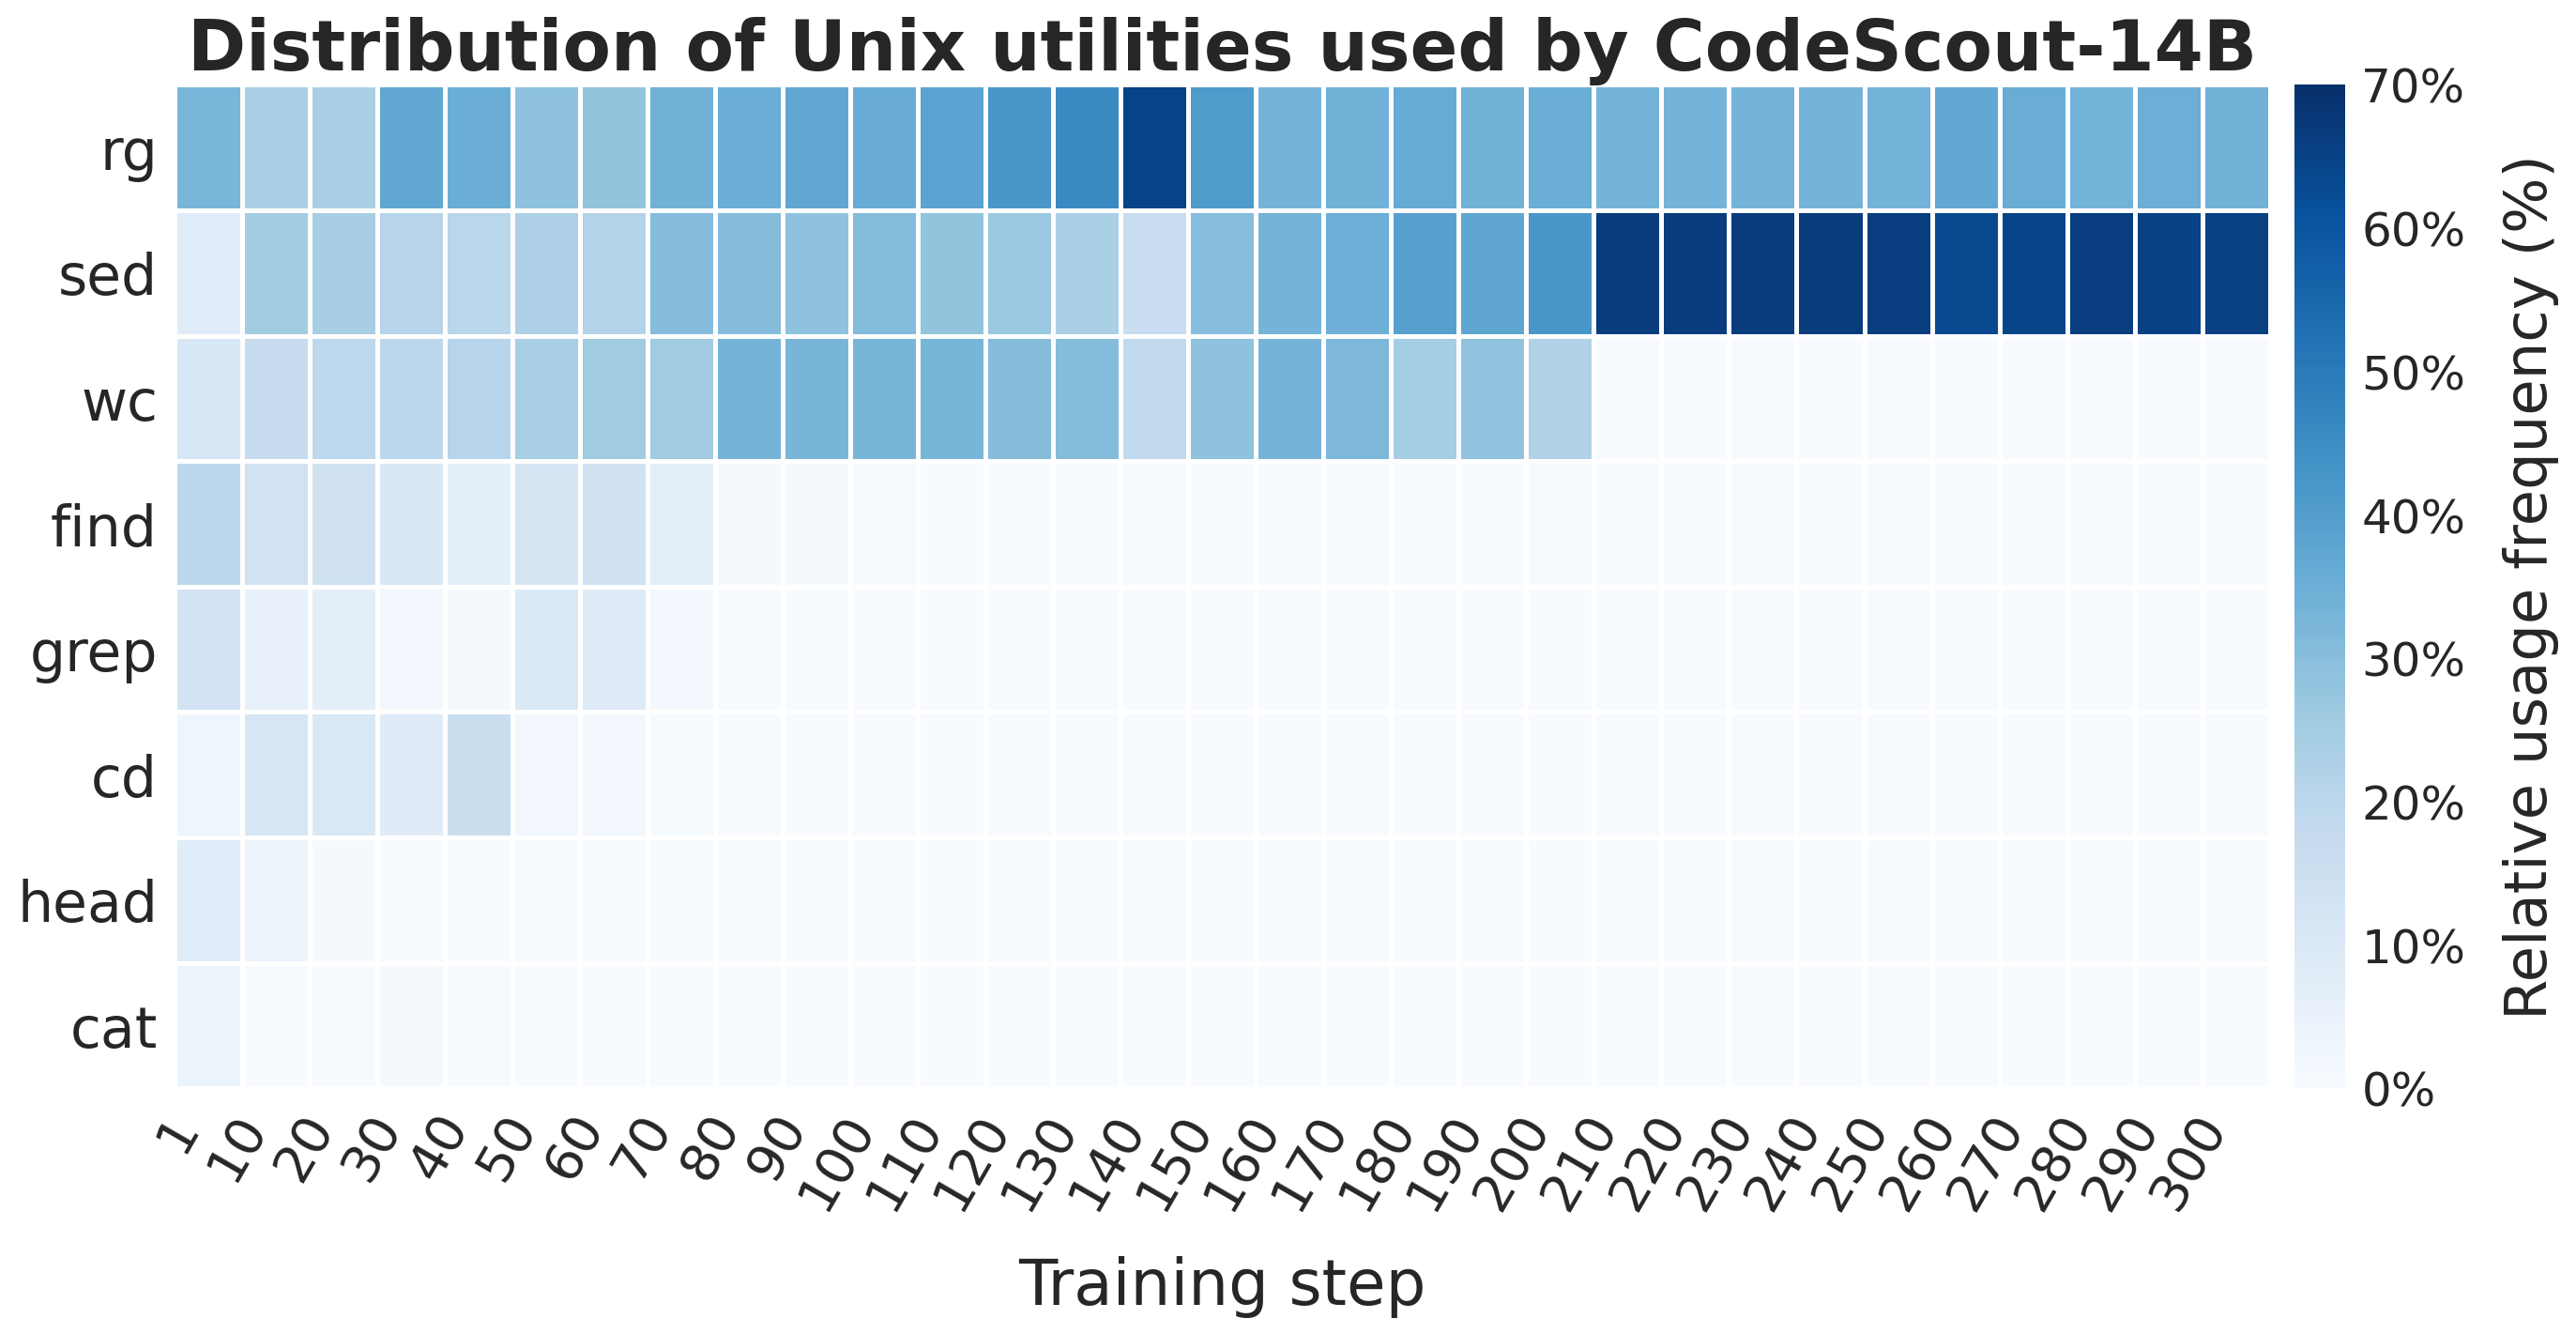
\includegraphics[width=\linewidth, height=\figheight]{Figures/command_relative_freq_14b.png}
        \caption{Tool use for \methodname-14B}
        \label{fig:tool_use_14b_sub}
    \end{subfigure}
    \hfill
    \begin{subfigure}[b]{\figwidth}
        \centering
        % Specifying both height and width forces the images to match exactly
        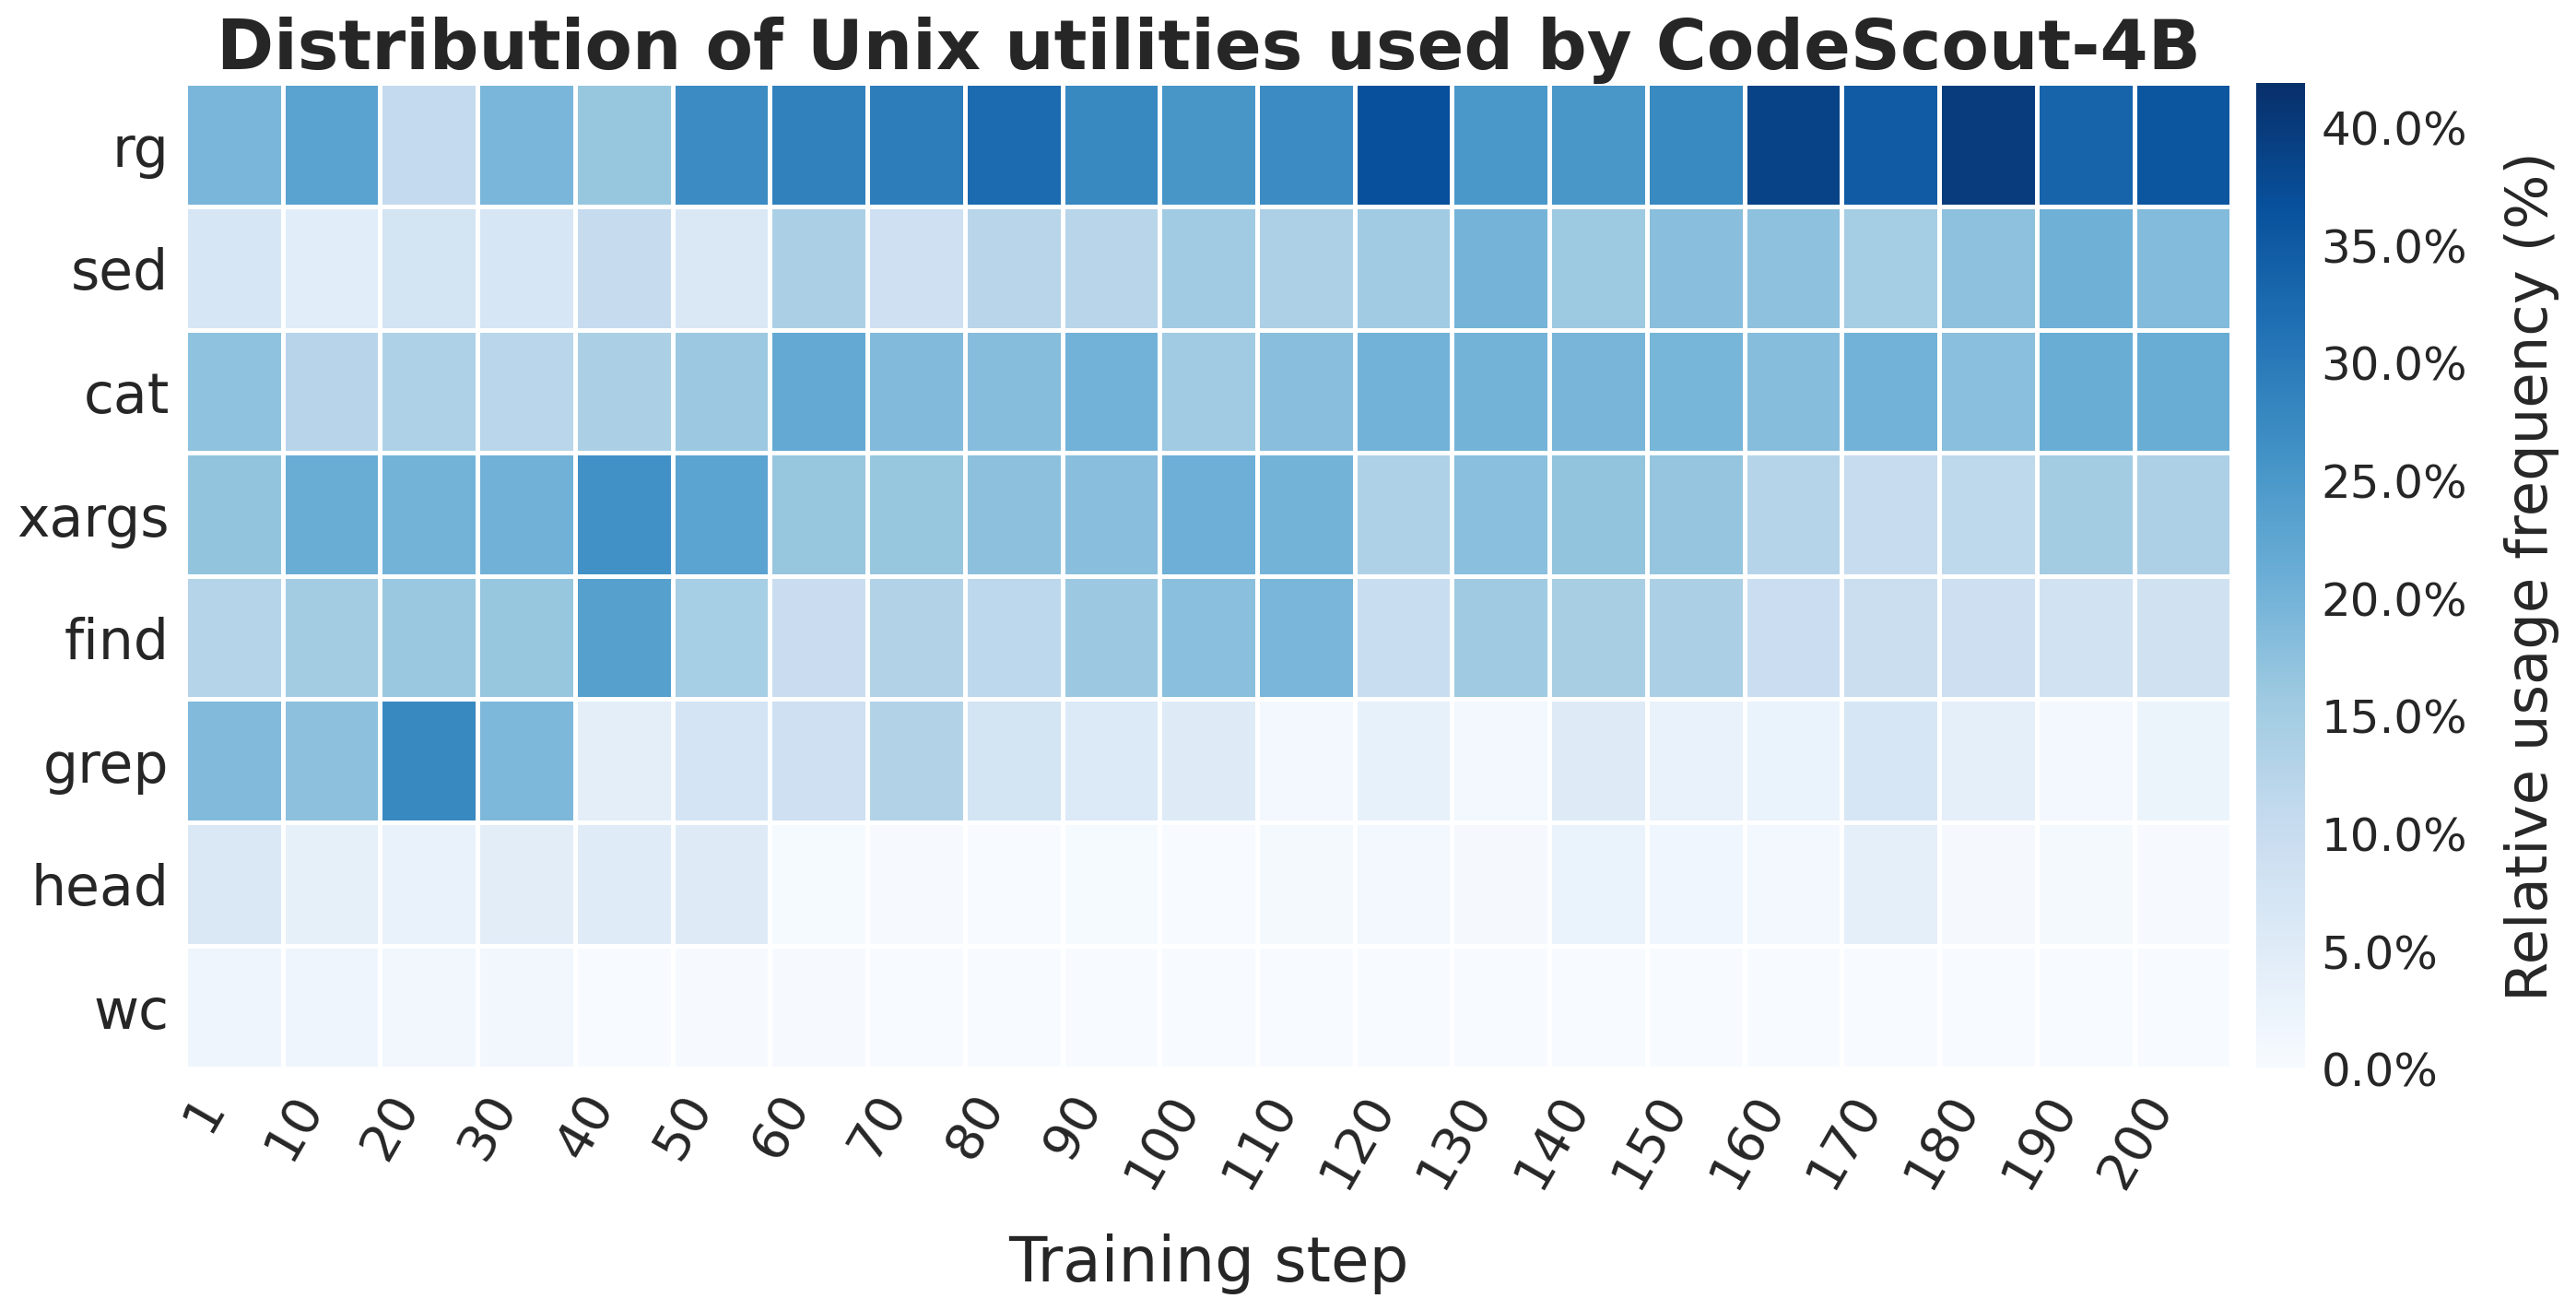
\includegraphics[width=\linewidth, height=\figheight]{Figures/command_relative_freq_4b.png}
        \caption{Tool use for \methodname-4B}
        \label{fig:tool_use_4b_sub}
    \end{subfigure}


    \caption{Distribution of the top-8 most frequent commands used by \methodname. LLMs start with diverse utilities and converge to a small set as training proceeds. \methodname-14B uses only ripgrep (rg) and sed, while \methodname-4B mainly uses rg, cat, sed, and xargs.}
    \label{fig:merged_tool_use}
\end{figure*}

% \begin{figure}[h]
%     \centering
%     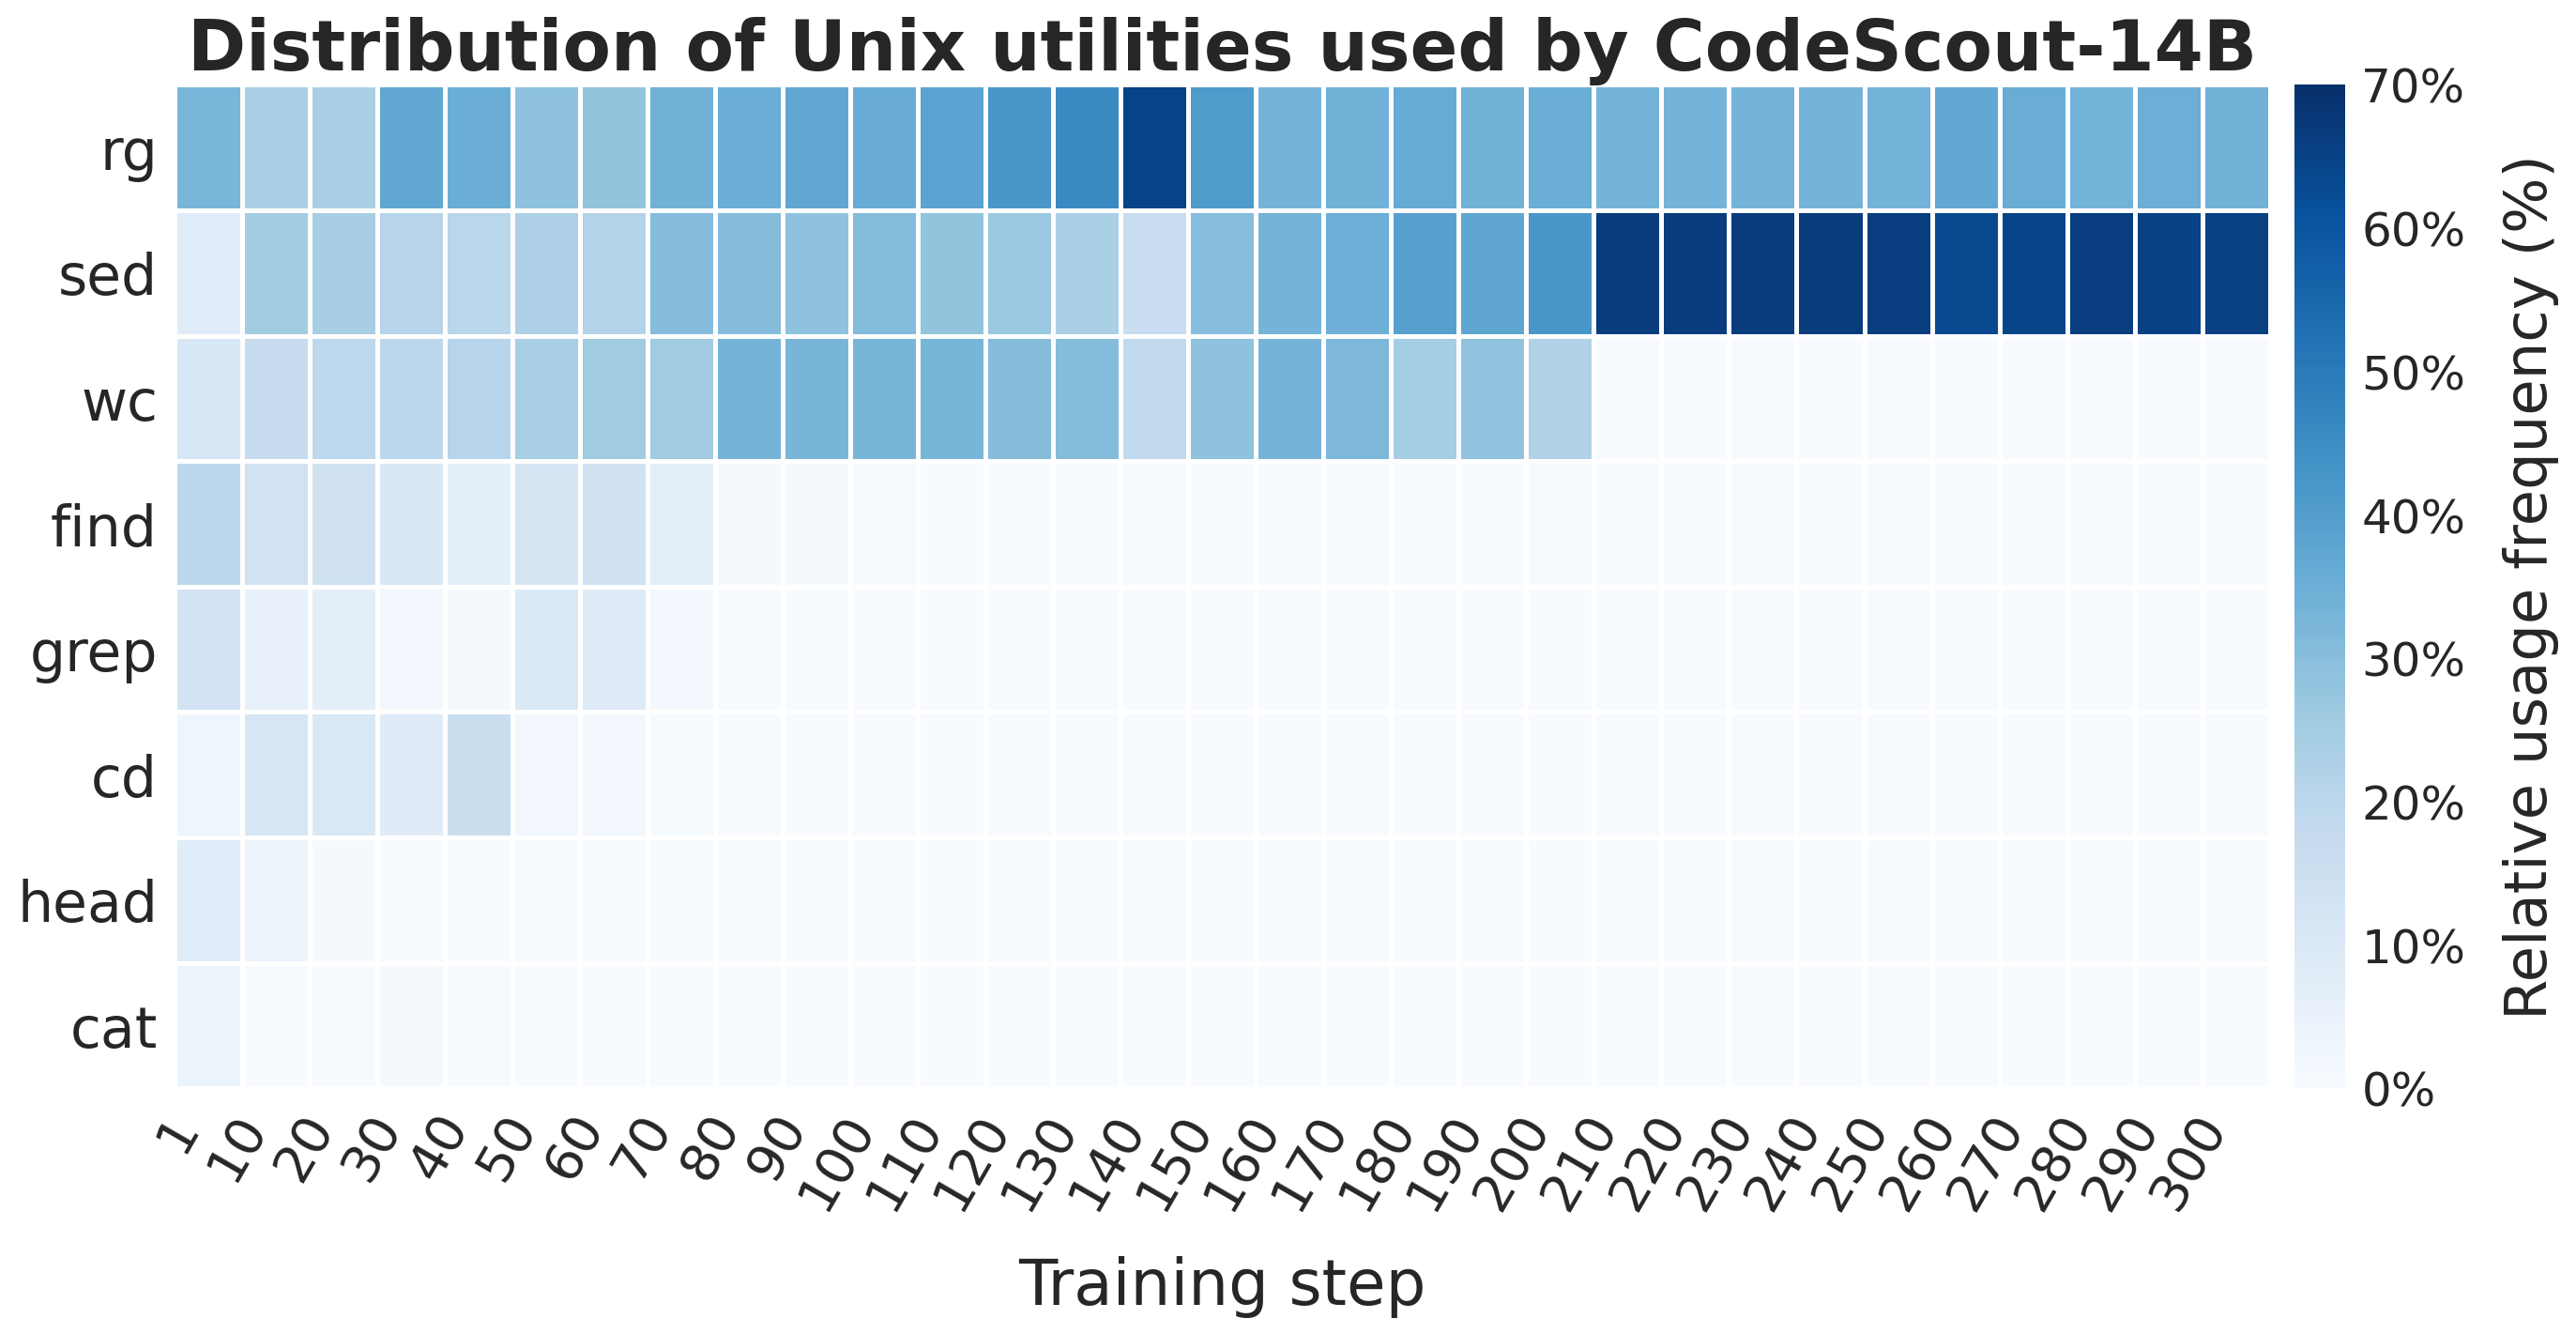
\includegraphics[width=\columnwidth]{Figures/command_relative_freq_14b.png}
%     \caption{Distribution of the top-8 most frequent Unix commands used by \methodname-14B measured using the relative usage frequency at different training steps during RL. \methodname-14B eventually converges to using just just two Unix commands, ripgrep and sed, and yet achieves strong code localization results.}
%     \label{fig:tool_use}
% \end{figure}
